% -----------------------------------------------
% Vlastní text práce (kapitoly práce)
% -----------------------------------------------

% -----------------------------------------------
\chapter{Gamma rays properties and matter interaction}
% -----------------------------------------------
\label{gammas}

% -----------------------------------------------
\section{Gamma radiation emission}


Gamma rays are photons, but the main difference from X-ray photons is that they originate only from the atomic nucleus when it is de-excited from a higher energy level to a lower one. The energy levels of the nucleus are similar to the levels in the electron shell - discrete, characteristic for each isotope and can be described by quantum numbers. Alpha and beta decays produce a new nucleus in an excited state and are therefore followed by gamma emission.

%Gamma rays are photons, but the mayor difference to the X-Ray photons is that they originate only from atomic nucleus upon its deexcitation from higher energy level to lower. The energy levels of nucleus are similar to the levels in electron shell - discrete, characteristic for every isotope and can be described by quantum numbers. Alpha and beta decays create a new nucleus in excited state, and thus they are followed by gamma emission.

%The gamma emission usually follows alpha or beta decays. The gamma photon is emitted due to the fact, that the new nucleus is created in an excited state.


% -----------------------------------------------
\section{Passage of radiation and particles through matter}
Interaction of a particle (radiation) with another particle (atom, nucleus) or with condensed matter can result in many types of interactions and effects - scattering of a particle, creation of new particles and nuclei, annihilation of the incident particle, etc. It depends mainly on the energy, electric charge, spin and mass of the particle, but also on the properties of the target particle or matter. The physical quantity that describes the probability of a particular interaction between a particle and a target is known as the cross section. Normalised to the unit solid angle - differential cross section:
%Interaction of a particle (radiation) with another particle (atom, nucleus) or with condensed matter can result into many types of interactions and effects - scattering of a particle, creation of new particles and nuclei, annihilation of incident particle etc. It mainly depends on particle's energy, electric charge, spin and mass, but also on the properties of target particle or matter. The physical quantity describing the probability of a specific interaction of particle with target is known as the cross section. Normalized to the unit solid angle - differential cross section:
 \begin{equation}
\frac{d\sigma}{d\Omega} = \frac{1}{F_{\textrm{part}}} \frac{dN_\textrm{s}}{d\Omega},
 \end{equation}
where $F_{\textrm{part}}$ is the particle flux, $\Omega$ is the solid angle and $N_\textrm{s}$ is the average number of particles scattered per unit time. And the total cross section is given by integration:
%where $F$ is a particle flux, $\Omega$ is a solid angle and $N_\textrm{s}$ is the average number of scattered particles per unit time. And the total cross section is given by integration:
  \begin{equation}
 \sigma = \int \frac{d\sigma}{d\Omega} d\Omega.
 \end{equation}


However, to characterise the interaction probability of a particle with condensed matter containing many interaction centres (defined by their density), other assumptions have to be made. The average number of scattered particles is given by:
%However, to characterize the interaction probability of particle with continuous matter, which contains many interaction centres (defined by their density), other assumptions have to be made. The average number of scattered particles is given by:
 \begin{equation}
 N_{\textrm{sc}}(\Omega) = F_{\textrm{part}}AN_{\textrm{i}} \delta x \frac{d\sigma}{d\Omega}
 \end{equation}
and integrated over the entire solid angle:
 \begin{equation}
 N_{\textrm{tot}} = F_{\textrm{part}}AN_{\textrm{i}}\sigma \delta x.
 \end{equation}
The $A$ is the total area perpendicular to the flux, $\delta x$ is the material thickness and $N_{\textrm{i}}$ is the density of interaction centres.
\par
Heavy charged particles (such as alpha particles, protons, muons, pions) lose energy mainly through collisions with atomic electrons. Due to their mass, which is much higher than the mass of the electrons ($M >> m_\textrm{e}$) they collide with, the direction of their trajectory remains unchanged. The energy loss per unit distance is defined as the stopping power $\frac{dE}{dx}$. The stopping power for the heavy charged particles is given by the Bethe-Bloch formula, which relates the stopping power to the energy of the particle. However, the Bethe-Bloch formula doesn't apply at low energies (guided by Lindhard theory) and at higher energies (bremsstrahlung radiation). The change in path direction is possible, with a lower probability, by the secondary interaction - elastic scattering from nuclei.
\par
Electrons and positrons have a much lower mass than the heavy charged particles, so the direction of their trajectory is changed by their movement in the electric field of the nucleus. The bremsstrahlung radiation losses are major yet at low energies. However, the energy lost in the collisions is also important - it is guided by the special Bethe-Bloch formula that takes into account the change in the direction of the path. 
\par
Other interaction effects are also possible (Cherenkov emission, nuclear reactions), but they are rare or do not affect the energy of the particle as much as those mentioned above. The interaction of neutrons is completely different because they have no charge. The interaction effects for gamma rays are described in more detail in the following chapter.  
%Heavy charged particles (such as alpha particles, protons, muons, pions) lose their energy mainly because of the atomic electrons collisions. Due to their mass which is much higher than the mass of electrons ($M >> m_\textrm{e}$) they collide with, the direction of their path is left unchanged. The loses of energy per unit path is defined as stopping power $\frac{dE}{dx}$. The stopping power for the heavy charged particles is given by Bethe-Bloch formula which relates stopping power and particle's energy. However the Bethe-Bloch formula doesn't apply at low energies (guided by Lindhard theory) and at higher energies (bremsstrahlung radiation). The change of their path direction is possible by the secondary interaction with lesser probability - by the elastic scattering from nuclei.
%\par
%Electrons and positrons have much smaller mass than the heavy charged particles, and thus the direction of their path is changed due to the movement in an electric field of nucleus. The bremsstrahlung radiation losses are major yet at low energies. However, the energy lost due to the collisions also comes to play - it is guided by special Bethe-Bloch formula, which takes the path direction change into account. 
%\par
%Other interaction effects are also possible (Cherenkov radiation emission, nuclear reactions), but they are rare or does not affect the particle's energy as those previously mentioned. The interaction of neutrons is totally different due to the lack of charge. The interaction effects for gamma rays are described more detail in the following chapter.



\subsection{Gamma matter interaction}
Due to the fact that gamma rays are photons, the gradual loss of kinetic energy within materials (characteristic of charged particles) is not observed. Instead, the main effect observed is the attenuation of the intensity of the photon flux with increasing thickness of the absorber material. 
%Due to the fact that the gamma rays are photons, the gradual losses of kinetic energy inside materials (characteristic for the charged particles) are not observed. Instead, the main observed effect is the attenuation of intensity of photon flux with the increasing thickness of the absorber material. 

\par
Three main interactions of photons with matter are: photoelectric effect, Compton scattering and pair production. The cross sections of these interactions vary with the gamma photon energy, the material and its density (strong dependence on the atomic number $Z$). Nuclear resonance interactions such as the Mössbauer effect are also possible, but their observation requires very special conditions.
%Three main interactions of photons with matter are: photoelectric effect, Compton scattering and pair production. The cross section of these interactions vary with gamma photon energy, with material and its density (high dependence on atomic number $Z$). The nuclear resonance interactions such as the Mössbauer effect are also possible, but their observation requires very special conditions to be met.


\par
The attenuation of the photon flux has a form of exponential decay:
\begin{equation}
I_{\textrm{T}} = I_{0}exp(-\mu x),
\end{equation}
where $I_{0}$ is the incident radiation intensity, $I_{\textrm{T}}$ is the transmitted radiation intensity and the parameter $\mu$ is the total absorption coefficient, which describes the probability of interaction per unit length and is bounded with the total cross section of single atom $\sigma_{\textrm{A}}$ (combination of the cross sections of the three main effects) by the relation:
\begin{equation}
 \mu = N_{\textrm{d}} \sigma_{\textrm{A}} = \sigma_{\textrm{A}}(N_{a}\rho/A_{\textrm{w}})
 \end{equation}
where $N_{\textrm{d}}$ is the atomic density, $N_{\textrm{a}}$ is the Avogadro number, $\rho$ is the material density and $A_{\textrm{w}}$ is the molecular weight. The total cross section of the combined three main interactions as a function of photon energy for lead is shown in the figure \ref{cross}.
%where $N$ is the density of atoms, $N_{a}$ is the Avogadro number, $\rho$ is the material density and $A_{\textrm{w}}$ is the molecular weight. The total cross section of combined three main interactions in dependence on the photon energy for lead is shown in the Fig. \ref{cross}.
\begin{figure}[H]
 \centering
 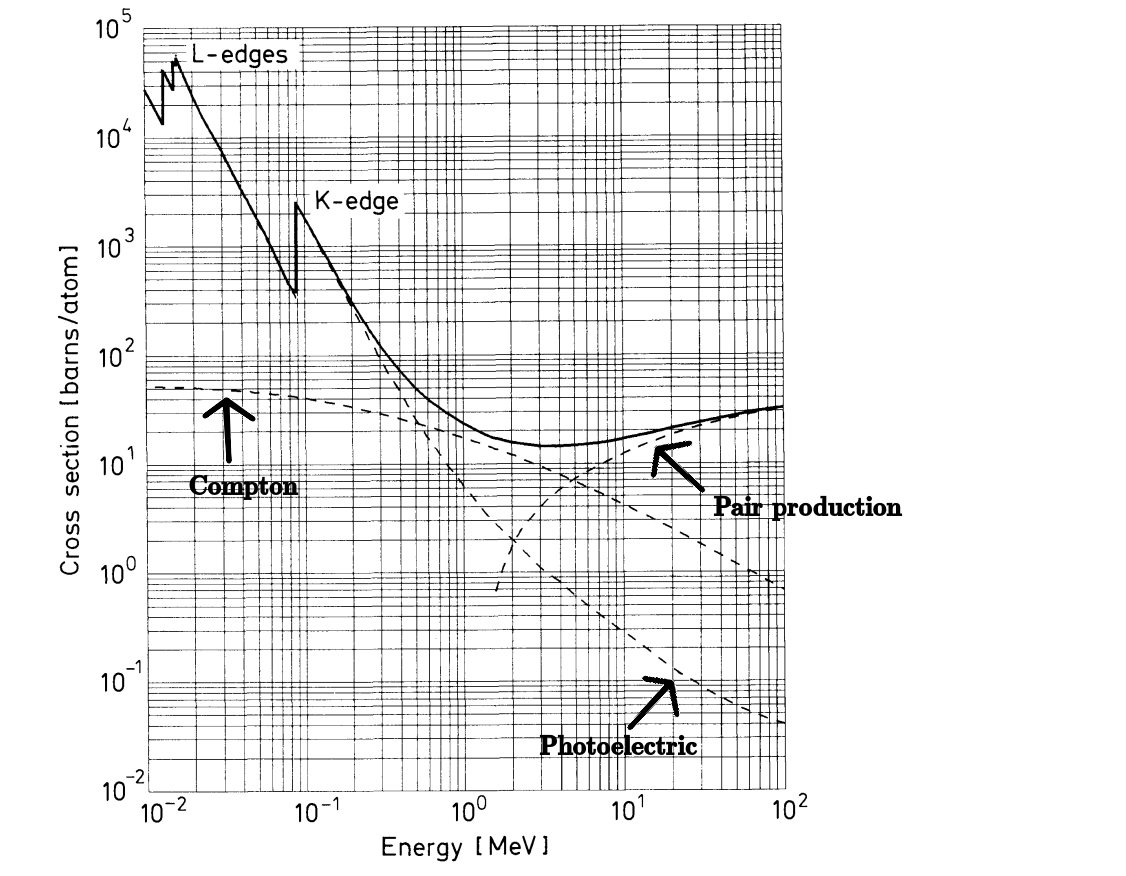
\includegraphics[scale=0.6, angle = 0]{./pictures/totalCross}
 \caption{Example of total absorption cross section for high energy photons for lead. Taken and modified from \cite{Leo1987-wy}.}
 \label{cross}
 
\end{figure}
 


\subsubsection{Photoelectric effect}
The photon is absorbed by an electron from the atomic shell. The electron is ejected and acquires the kinetic energy given by the well-known equation:
%The photon is absorbed by electron from atomic shell. The electron is ejected and acquires the kinetic energy given by well-known equation:
 \begin{equation}
 E_{\textrm{e}} = hf - E_{\textrm{b}},
 \end{equation}
where $f$ is the photon frequency and $E_{\textrm{b}}$ is the binding energy.
\par
The photoelectric effect can only be observed on electrons bounded in the atomic shell, because the nuclei can absorb the momentum of the photon. The cross section usually decreases with energy and can show characteristic discontinuities of K, L, M transitions. Two types of photoelectric effect can be distinguished - external and internal. External photoelectric effect results in the ejection of the electron out of the material - an effect observed in photocathodes. Internal photoelectric effect causes the electron to be excited to a higher energy level - in semiconductors this means from the valence band to the conduction band. The photoelectric effect plays a key role in the detection of gamma photons.
%The photoelectric effect can be observed only on electron bounded in atomic shell, due to the fact, that the nuclei can absorb the momentum of the photon. The cross section usually falls with energy and can exhibit characteristic discontinuities from K, L, M transitions. Two types of photoelectric effect can be distinguished - external and internal. External photoelectric effect results into ejecting the electron outside of the material - effect observed on photo cathodes. Internal photoelectric effect results into exciting the electron into the higher energy level - in semiconductor it means from the valence band to the conduction band. The photoelectric effect plays a key role when it comes to the detection of gamma photons.

\subsubsection{Compton scattering}
Compton scattering is an effect mainly observed on free electrons. It must be said that the electrons in a material are usually bound, but if the photon energy is much higher than the binding energy, the electron can be considered free \cite{Leo1987-wy}.
%Compton scattering is an effect, which is mainly observed on free electrons. It needs to be said, that the electrons in material are usually bounded, however, if the photon energy is much higher than the binding energy, the electron can be considered as free \cite{Leo1987-wy}.
\par
This effect causes the photon to lose only part of its energy and change direction. The energy is transferred to an electron according to the laws of conservation of energy and momentum, and can be described by the following relationship:
%This effect causes, that the photon loses only a part of its energy and changes its direction. The energy is transferred to an electron accordingly to the laws of energy and momentum conservation and can be described by following relation:
\begin{equation}
\begin{aligned}
E_{\textrm{e}} = E_1 - E_2 = E_1 [1- \frac{1}{1+\frac{E_1}{m_{\textrm{e}}c^2}(1 - \cos{\theta})}],
\end{aligned}
\label{compton}
\end{equation}
where $E_{\textrm{e}}$ is the energy transferred to an electron, $E_1$ is the initial photon energy, $E_2$ is the scattered photon energy, $m_{\textrm{e}}$ is the the electron mass and $\theta$ is the scattering angle. This equation can be used to calculate the positions of Compton edges in energy spectra by plugging in the angle of maximum energy transfer ($\varphi = 180^\circ$).


\subsubsection{Pair production}
At much higher energies, the photon can be converted into an electron-positron pair. This effect occurs near the nucleus, which absorbs a part of the original photon momentum \cite{Leo1987-wy}. Minimum required energy is 1.022 MeV, which corresponds to 2$\times$ electron rest energy.
%At much higher energies, the photon can be converted into electron-positron pair. This effect happens near the nucleus, which absorbs a part of the original photon momentum \cite{Leo1987-wy}.
\par
The pair production and the electron bremsstrahlung are key effects in the development of electron-photon showers. If the electron/positron produced has sufficient energy, it emits bremsstrahlung photons. These bremsstrahlung photons can interact again via pair production, creating new electrons. This process of shower evolution continues until the energy of the electron/positron pairs falls below the energy required to produce bremsstrahlung radiation. At lower energies, the electrons lose more of their energy through atomic collisions than through bremsstrahlung.
\par
Negative effects from this type of interaction, such as the creation of single and double escape peaks or annihilation peaks in spectra, are not observed because the cross section for low-energy gamma photons is very small. This means that this interaction can be neglected for the purposes of this thesis. 
%The pair production along with electron bremsstrahlung radiation  are key effects for electron-photon shower development. If the created electron/positron has sufficient energy, it emits bremsstrahlung photons. These bremsstrahlung photons can interact again via the pair production, thus creating new electrons again. This process of shower development continues until the energy of electron/positron pairs drops under the energy, which is required to produce bremsstrahlung radiation. At lower energies, the electrons lose more of their energy through the atomic collisions rather than through bremsstrahlung.
%\par
%Negative effects arising from this type of interaction like creation of single and double escape peaks or annihilation peaks in spectra will not be observed because for low-energy gamma photons the cross-section is very small. That means that for the purposes of this thesis, this interaction could be neglected.   


\subsection{Characteristic energy spectra}
\label{char}
Each gamma source emits photons with a characteristic energy with a certain probability. However, this characteristic energy can be altered by interactions that may occur in the environment or within the detector itself. This results in the registration of photon events with altered energies.
%Every gamma source emits photons with characteristic energies with certain probabilities. However, this characteristic energy can be altered by the interactions, which can occur in environment or inside the detector itself. That results into registration of photon events with altered energies.
\par
In the environment the energy spectra can be affected by:
\begin{itemize}
\item Characteristic X-rays - radiation-induced fluorescence usually from the shielding material (Pb).
\item Backscatter peak - Compton scattering which occurred over a wide angle.
\end{itemize}
\par
Inside the detector the energy spectra can be affected by:
\begin{itemize}
\item X-ray escape peaks - When the photoeffect occurs at atomic energy levels, the characteristic X-ray of the detector material is emitted. The escape peak has the energy of the captured photon minus the energy of the escaped X-ray.
\item Compton continuum - the photon interacts inside detector by Compton scattering, the scattered photon leaves the detector,  which registers the photon energy loss.
\end{itemize}

% %%%%%%%%%%%%%%%%%%%%%%%% End of file %%%%%%%%%%%%%%%%%%%%%%%%